%
% Motivation / Introduction
%
\section{Introduction}

The aim of this project is to develop a web-application which provides its user with access to a large collection of recipes. The website will use machine learning techniques to create visualisations of these recipes as a graph of nodes, encouraging the exploration of new ingredients and recipes.

The user will be able to submit their own recipes to the website and rate those they come across, allowing them to receive personalised recommendations of recipes they may be interested in. Furthermore, the user will be able to form "friendships" with other users to see the recipes that friends upload or like themselves.

The user can select several recipes to build a 'meal plan', which will have a corresponding shopping list containing the ingedients required to make these meals. 

%
% Aims, Objectives and deliverables.
%
\section{Aims, Objectives and Delievarables}

\subsection{Project Aims}
<A brief summary of the primary aims of this project. Typically 1-3 sentences.>

This project aims to incorporate web technologies and machine learning to produce a web-application delivering personalised recommendations to its users. 
Visualisation techniques will be used to display both the result of clustering recipe documents and the relationships between ingredients across different recipes.
\subsection{Objectives}

<A list of what you want to achieve {\em by the end of the project} -- note this means `learn how to\ldots', `research into\ldots` are {\em not} objectives, as they are intermediate milestones rather than final goals. All objectives should be measurable, {\em i.e.} it should be possible to provide evidence to confirm whether or not they have been achieved. 3-5 objectives is typical.>

- Identify if some features require additional time 

The objectives of this project involve developing:

\begin{itemize}
    \item A front-end for the web application
    \item A back-end for the web-application
    \item A machine learning backend API which delivers personalised user recommendations

\end{itemize}

\subsection{Deliverables}

%<A list of what you will hand in at the end of the project. This will include the final report (possibly spread across multiple deliverables, if that makes sense for your project), code (possibly more than one version), and so on. Ideally the deliverables should be cross-referenced to the objectives. 2-3 deliverables is typical, but there can be more depending on the nature of the project.>

The project will comprise the following deliverables:
\begin{itemize}
    \item A repository containing the code for the web application, including:
        \begin{itemize}
            \item A web front-end which displays the application's data and allows the user to interact with the backend APIs
            \item A web back-end API which delivers the data required to render the front-end
            \item A machine-learning backend API which delivers personalised user recommendations 
        \end{itemize}
    \item A final report summarising the development of the codebase
\end{itemize}

%   
% Plan
%
\section{Project Plan}

%<Provide a plan for the full project, from when you started until the submission of the final report. This should discuss the key stages of your project.>

A plan is given for each distinct part of the project. These plans will be executed simultaneously.


\textbf{Web Front-End}
\begin{itemize}
    \item Identify web-pages using user stories
    \item Identify required end-points for each web-page
    \item Identify framework to use
    \item Research graph visualisation on web-pages
    \item Develop front-end components
\end{itemize}
\textbf{Web Back-End}
\begin{itemize}
    \item Identify framework to use
    \item Develop endpoints identified in Front-End Development
\end{itemize}
\textbf{Machine Learning Recommendation}
\begin{itemize}
    \item Research recommendation systems
    \item Implement different approaches
    \item Evaluate performance
    \item Make accessible to web backend
\end{itemize}

\subsection{Timeline}

<A graphical description of your plan, often as a Gantt chart.>

% To include a figure, uncomment and modify the following. Vary the 'width'
% field until it looks suitable. This uses the 'graphicx' module that has
% already been included in 'config.tex'.
\begin{figure}[htbp]	
	\centerline{
		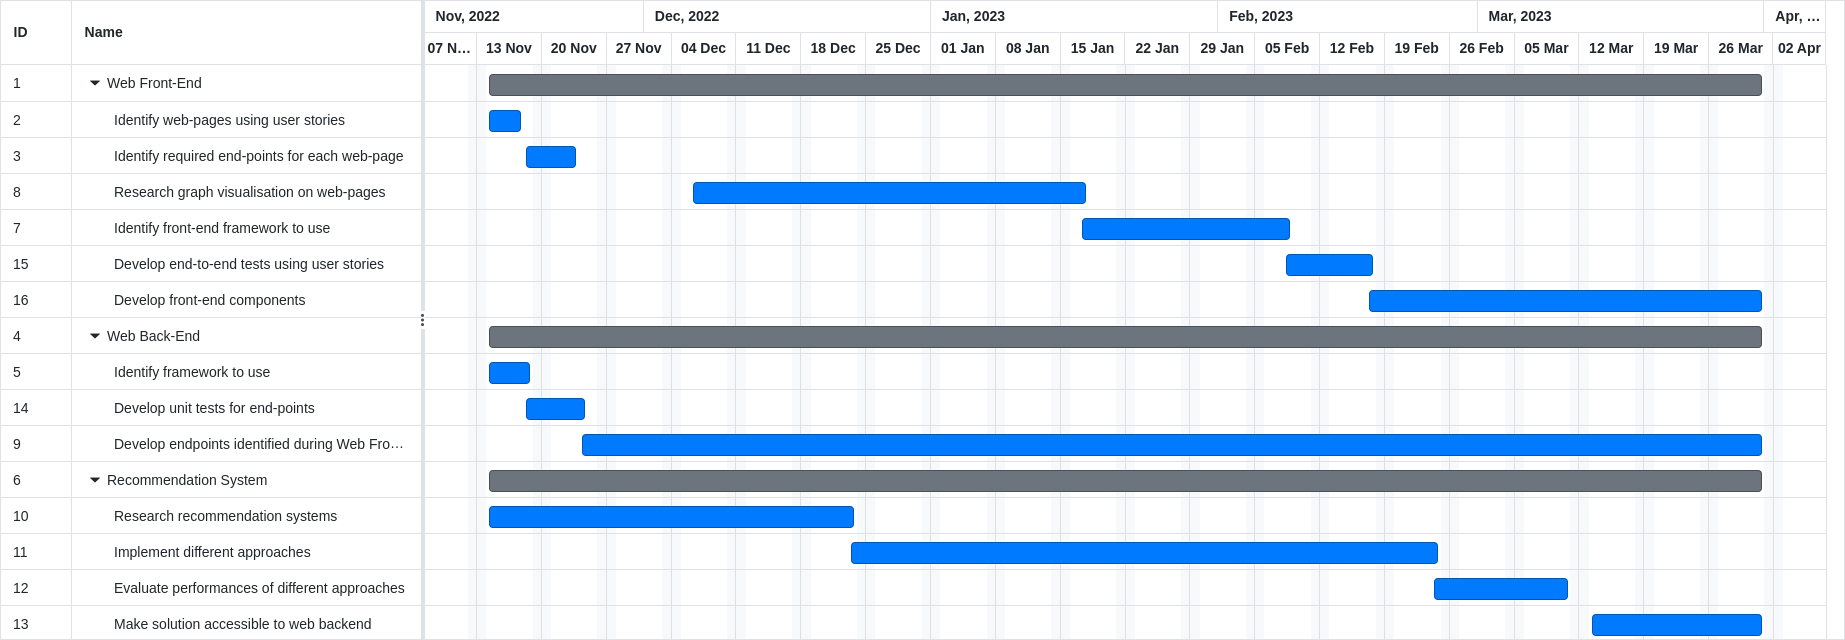
\includegraphics[width=10cm]{../PlanGantt.png}
	}
	\caption{Gantt Chart Depiction of Project Plan}
\end{figure}



%
% Risk mitigation.
%
\section{Risk Mitigation}

<Identify risks to your project, and what you would do if they arose.>

The project's development faces several risks:
\begin{itemize}
    \item Rendering the graph visualisations
        \begin{itemize}
            \item There is a large amount of data so optimising for performance may be difficult.
            \item It's unclear how many existing solutions exist that could be suitably adapted for the task at hand to ensure all desired functionality is met.
        \end{itemize}
    \item Machine learning recommendation
        \begin{itemize}
            \item Machine learning has few guarantees and it's certainly feasible that a recommendation system may deliver unsatisfactory recommendations.
        \end{itemize}
\end{itemize}

%
% Ethics.
%
\section{Ethics}

There are several ethical issues involved in the project:
\begin{itemize}
\item Collection of user data - personal data including email addresses and passwords will be collected, alongside inferences made about users' preferences.

This will be mitigated by ensuring the project complies with the Data Protection Act, storing and deleting user data as required. 
\item The project involves a large quantity of unmoderated data. It will include systems that allow for the submission of new text which will become publicly available to others using the application. 

This risk will be mitigated by allowing users to report offensive content, flagging it for review and potential removal.
\item The project allows users to indirectly interact with others through a friendship system and submission of unmoderated content.

To ensure that users can prevent unwanted communication from others, they will be able to block other users from making any direct or indirect communicaton with them.
\end{itemize}